\documentclass[tikz,dvisvgm]{standalone}

\usetikzlibrary {positioning,arrows.meta,fit,backgrounds}

\pgfdeclarelayer{coders}
\pgfdeclarelayer{layers}
\pgfdeclarelayer{containers}
\pgfsetlayers{coders,layers,containers,main}

\begin{document}
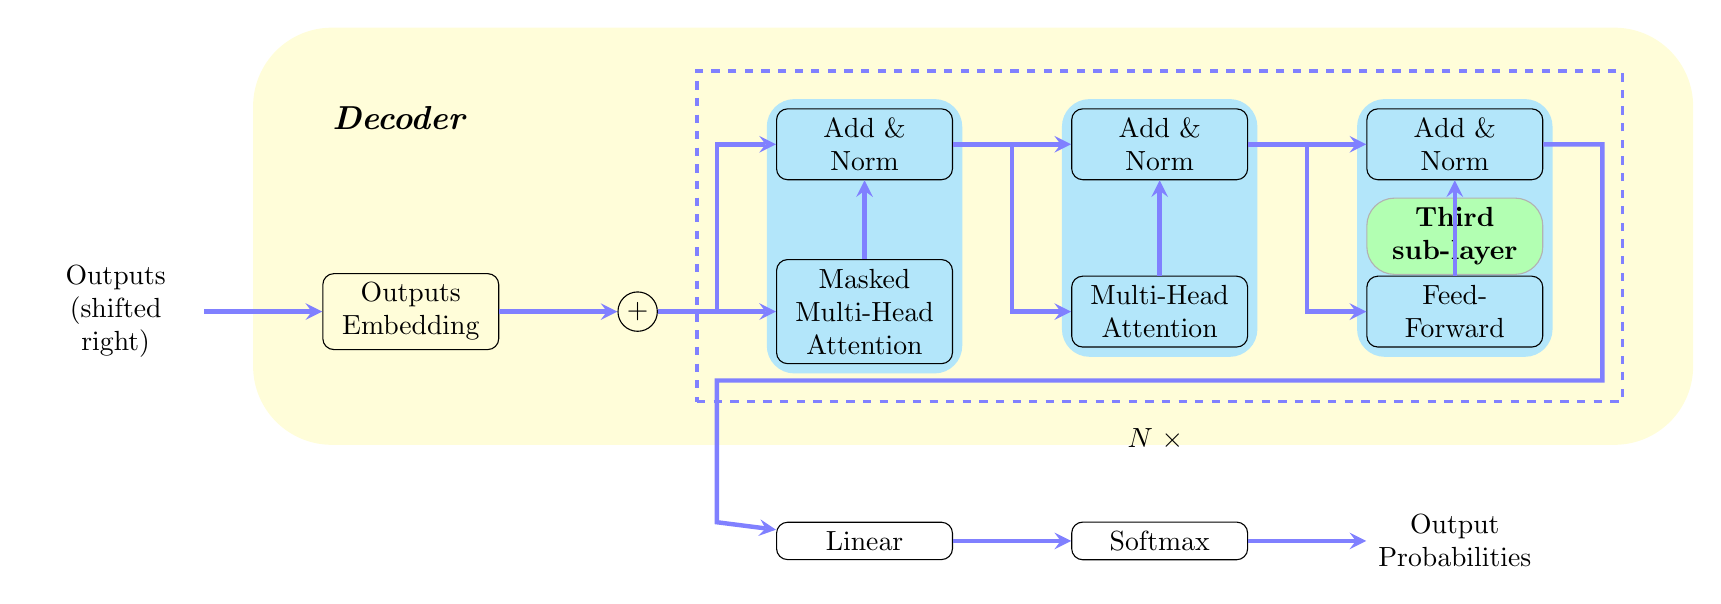
\begin{tikzpicture}[
    every text node part/.style={align=center,text width=2cm,},
    nn/.style = {draw,rectangle,rounded corners},
    arr/.style = {draw=blue!50, ultra thick},-stealth,
    plus/.style= {draw,circle,inner sep=0pt,minimum size=0.5cm,text width=0cm,align=center},
    conn/.style = {draw=blue!50, ultra thick},
    layer/.style = {fill=cyan!30, rounded corners=10pt},
    container/.style = {draw=blue!50, dashed, very thick, inner xsep=25pt, inner ysep=10pt},
    coder/.style = {inner xsep=25pt, inner ysep=15pt, rounded corners = 1cm},
    layertext/.style = {fill=green!30,draw=black!30,rectangle,rounded corners=10pt,font=\bfseries},
    node distance = 1cm and 1.5cm,
  ]

  \node (outputs) {Outputs \\ (shifted right)};
  \node [nn, right= of outputs] (outputs-embedding) {Outputs \\ Embedding};
  \node [plus, right= of outputs-embedding] (plus2) {};
  \node at (plus2) {+};
  \path[arr] (outputs) to (outputs-embedding);
  \path[arr] (outputs-embedding) to (plus2);

  \node [nn, right= of plus2] (masked-multi-head) {Masked \\ Multi-Head Attention};
  \node [nn, above= of masked-multi-head] (addnorm3) {Add \& Norm};
  \path [arr] (masked-multi-head) to (addnorm3);

  \begin{pgfonlayer}{layers}
    \node [layer, fit=(masked-multi-head) (addnorm3)] (sublayer3) {};
    % \node [above=0.2cm of sublayer3] (secondsublab) {First sub-layer};
  \end{pgfonlayer}

  \coordinate[right=0.75cm of plus2] (aux3);
  \path[arr] (plus2) to (masked-multi-head);
  \path[arr] (aux3) |- (addnorm3);

  \node [nn, right= of addnorm3] (addnorm4) {Add \& Norm};
  \node [nn] (multi-head2) at (addnorm4 |- masked-multi-head) {Multi-Head \\ Attention};

  \begin{pgfonlayer}{layers}
    \node [layer, fit=(multi-head2) (addnorm4)] (sublayer4) {};
    % \node at (sublayer4 |- secondsublab) {Second sub-layer};
  \end{pgfonlayer}

  \path[arr] (multi-head2) to (addnorm4);
  \coordinate[right=0.75cm of addnorm3] (aux4);
  \path[arr] (addnorm3) to (addnorm4);
  \path[arr] (aux4) |- (multi-head2);

  \node [nn, right= of addnorm4] (addnorm5) {Add \& Norm};
  \node [nn] (feed-forward2) at (addnorm5 |- multi-head2) {Feed-Forward};
  \path [arr] (feed-forward2) to (addnorm5);

  \coordinate[right=0.75cm of addnorm4] (aux5);
  \path[arr] (addnorm4) to (addnorm5);
  \path[arr] (aux5) |- (feed-forward2);

  \begin{pgfonlayer}{layers}
    \node [layer, fit=(feed-forward2) (addnorm5)] (sublayer5) {};
    \node [layertext] at (sublayer5 |- sublayer3) {Third sub-layer};
  \end{pgfonlayer}

  \begin{pgfonlayer}{containers}
    \node [container, fit=(sublayer3) (sublayer4) (sublayer5)] (decoder) {};
    \node [below=0.2cm of decoder] {$N \times{}$};
  \end{pgfonlayer}

  \begin{pgfonlayer}{coders}
    \node [fill=yellow!15, coder, fit=(decoder) (plus2) (outputs-embedding)] (decoder-container) {};
    \node [left=-3cm of decoder-container, yshift=1.5cm] (decoderlab) {\large \textbf{\textit{Decoder}}};
  \end{pgfonlayer}

  \node [nn, below=2cm of masked-multi-head] (linear) {Linear};
  \node [nn, right= of linear] (softmax) {Softmax};
  \node [right= of softmax] (proba) {Output Probabilities};

  \coordinate[right=0.75cm of addnorm5] (aux10);
  \coordinate [below=3cm of aux10] (aux11);
  \coordinate (aux12) at (aux3 |- aux11);
  \coordinate [below=1.8cm of aux12] (aux13);

  \draw [conn] (addnorm5) to (aux10) to (aux11) to (aux12) to (aux13) to (linear);

  \path[arr] (linear) to (softmax);
  \path[arr] (softmax) to (proba);
\end{tikzpicture}

\end{document}